% -*- coding: utf-8 -*-
\documentclass[12pt]{article}
\usepackage{amssymb}%为了打印出反斜杠
\usepackage{listings}
\usepackage{ctex}
\usepackage{graphicx}
\usepackage[a4paper, body={18cm,22cm}]{geometry}
\usepackage{amsmath,amssymb,amstext,wasysym,enumerate,graphicx}
\usepackage{float,abstract,booktabs,indentfirst,amsmath}
\usepackage{array}
\usepackage{booktabs} %调整表格线与上下内容的间隔
\usepackage{multirow}
\usepackage{diagbox}
\usepackage{color}%字体颜色包
\usepackage[colorlinks,linkcolor=blue,urlcolor=black,anchorcolor=blue,citecolor=blue,]{hyperref}%超链接包
\usepackage{amssymb}%为了打印出反斜杠
\renewcommand\arraystretch{1.4}
\usepackage{indentfirst}
\setlength{\parindent}{2em}

\geometry{left=2.8cm,right=2.2cm,top=2.5cm,bottom=2.5cm}
%\geometry{left=3.18cm,right=3.18cm,top=2.54cm,bottom=2.54cm}

\graphicspath{{figures/}}

\title{\heiti 实验六:PyTorch下的神经网络训练用于AGAC的实体识别}

\begin{document}

	\maketitle
	
	\vspace{5cm}
	
	\begin{table}[h]
		\centering
		\begin{Large}
			\begin{tabular}{p{3cm} p{7cm}<{\centering}}
				学  \qquad  校: &  华中农业大学     \\ \cline{2-2}
				学院班级:      & 信息学院生信1801班   \\ \cline{2-2}
				姓  \qquad  名: & 邓启东 \\ \cline{2-2}
				学  \qquad  号: & 2018317220103 \\ \cline{2-2}
				指导教师:       &夏静波 \\ \cline{2-2}
			\end{tabular}
		\end{Large}		
	\end{table}
	
	\newpage%一个新的页面

	\tableofcontents
	
	\newpage
	\section{实验目的}
\subsection{LSTM+CRF}
本次实验采用LSTM+CRF这套代码,依旧完成AGAC实体识别task1。通过LSTM+CRF的方式弥补单用LSTM本身无法对标签转移关系进行建模的问题。在LSTM+CRF模型中,前一类特征函数的输出由LSTM的输出替代,后一类特征函数就变成了标签转移矩阵。
\section{数据处理}
\subsection{数据处理前后格式}
首先我们从Github上将项目下载下来。\par
一开始语料库是jason格式,通过运行json2bio.py代码将AGAC\_train和AGAC\_answer这两个压缩包的据转换为BIO格式,分别得到train.txt,valid.txt,test.txt。他们的内容都是单个的分词加上反斜杠再加上其标签,以空格分隔开每个词语(见图\ref{sdasad}),至此数据准备完毕。\par
\begin{figure}[H]
  \centering
  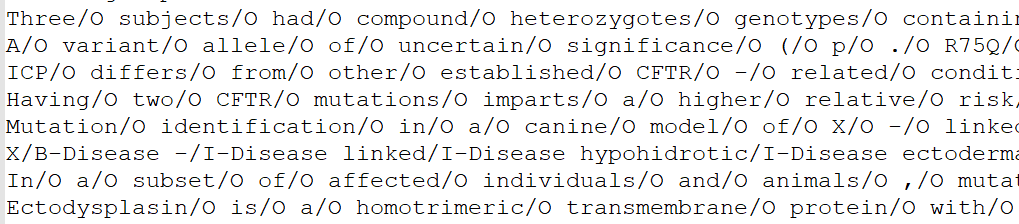
\includegraphics[scale=0.4]{./picture/data.png} %1.png是图片文件的相对路径
  \caption{处理后数据格式} %caption是图片的标题
  \label{sdasad} %此处的label相当于一个图片的专属标志,目的是方便上下文的引用
\end{figure}
\section{模型训练}
\subsection{训练前的处理}
在整个过程开始之前还要首先运行prepare.py文件。\par
将train.txt中的每一个分词分成标签,字符,以及单词。并且生成存储他们的Index的文件,分别为train.txt+ .char\_to\_idx/.word\_to\_idx/.tag\_to\_idx。\par
所有的参数设置可以在parameters.py找到。可以设置EMBED参数也就是embedding维数。\par
predict.py:(第16行)的load\_checkpoint('model.epoch20', model)表示多少步长打印一下结果。\par
train.py: num\_epochs = 20也是步长检查一下训练效果。\par
运行train.py开始训练。这一步会得到训练好的模型并打印出模型结构。
\subsection{出错与解决}
出现报错(见下图\ref{111}):
\begin{figure}[H]
  \centering
  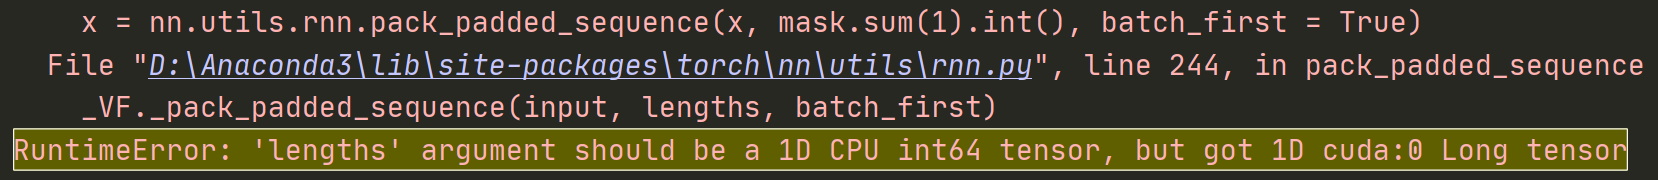
\includegraphics[scale=0.4]{./picture/error.png} %1.png是图片文件的相对路径
  \caption{报错} %caption是图片的标题
  \label{111} %此处的label相当于一个图片的专属标志,目的是方便上下文的引用
\end{figure}
解决问题:\par
可以发现以上报错内容提示,参数“lengths”应该使用CPU int64,经过查阅出现以上报错的原因可能是由于Pytorch版本的问题,不能使用GPU版本进行代码的运行,此时,可以改用CPU进行代码尝试。\par
解决方法:\par
直接在报错指定的地方改成CPU进行运算。即调用 .cpu() 直接添加在报错参数的后面。也就是在模型的76行后面加.cpu()
(如下图\ref{sdasadf})。\par
\begin{figure}[H]
  \centering
  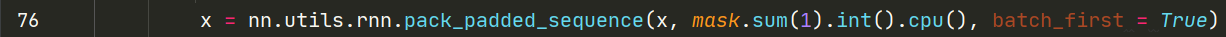
\includegraphics[scale=0.5]{./picture/fixerror.png} %1.png是图片文件的相对路径
  \caption{改成CPU运算} %caption是图片的标题
  \label{sdasadf} %此处的label相当于一个图片的专属标志,目的是方便上下文的引用
\end{figure}

可以看到随着模型的训练,loss越来越小,也就是模型的拟合效果越来越高(图\ref{aaaaa})。
\begin{figure}[H]
  \centering
  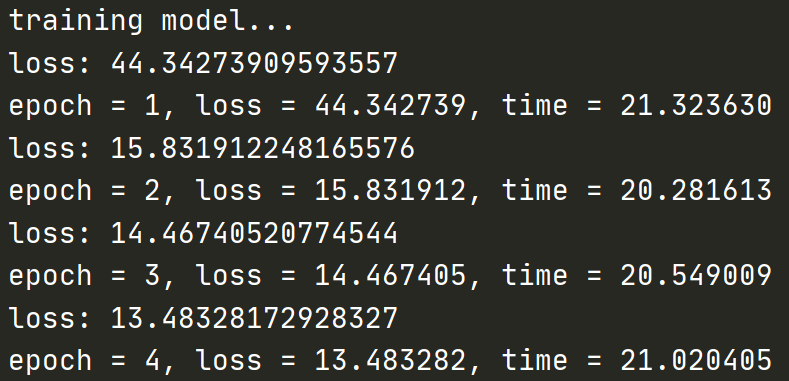
\includegraphics[scale=0.4]{./picture/loss.png} %1.png是图片文件的相对路径
  \caption{训练过程} %caption是图片的标题
  \label{aaaaa} %此处的label相当于一个图片的专属标志,目的是方便上下文的引用
\end{figure}
\subsection{模型保存}
最后到了30次epoch的时候,可以看到(见图\ref{dsfd})loss已经下降到了0.458291,已经非常小了,至此保存模型。
\begin{figure}[H]
  \centering
  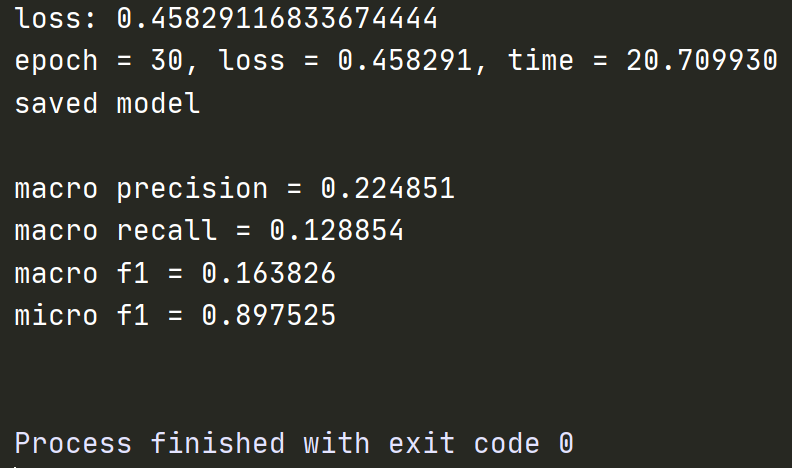
\includegraphics[scale=0.4]{./picture/loss2.png} %1.png是图片文件的相对路径
  \caption{模型训练完毕} %caption是图片的标题
  \label{dsfd} %此处的label相当于一个图片的专属标志,目的是方便上下文的引用
\end{figure}
\section{标签预测}
\subsection{报错与解决}
运行predict.py文件对标签进行预测,发现出现报错(见下图\ref{sssfqqqq})。
\begin{figure}[H]
  \centering
  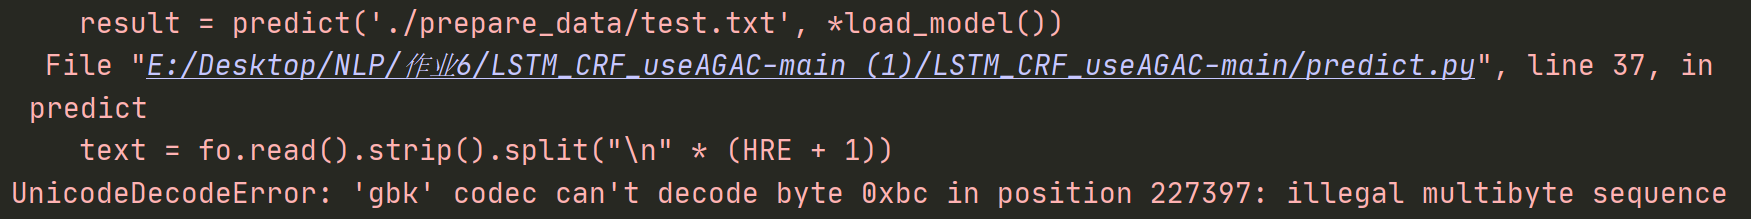
\includegraphics[scale=0.3]{./picture/error2.png} %1.png是图片文件的相对路径
  \caption{报错} %caption是图片的标题
  \label{sssfqqqq} %此处的label相当于一个图片的专属标志,目的是方便上下文的引用
\end{figure}
这个报错比较简单,就是打开文件的时候txt是utf-8编码,所以编码需要转为utf-8,因此要在每一个文件打开的语句中间加上,encoding='utf-8'。分别在第31行和第61行添加上以后。报错解决
\subsection{预测完成}
看到下面的内容,说明预测已经完成了(图\ref{zzaa})。
\begin{figure}[H]
  \centering
  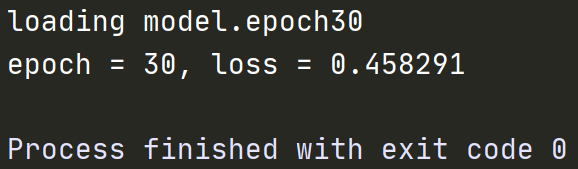
\includegraphics[scale=0.5]{./picture/predict.png} %1.png是图片文件的相对路径
  \caption{报错} %caption是图片的标题
  \label{zzaa} %此处的label相当于一个图片的专属标志,目的是方便上下文的引用
\end{figure}

\section{结果评估}
\subsection{github代码笔误}
评估代码如下:\par
perl conlleval.pl -d \$'$\setminus$t' <test\_out.tab | tee test\_out\_lstm.eval\par
却发生了报错,表明没有参数(见下图\ref{asjhal})。
\begin{figure}[H]
  \centering
  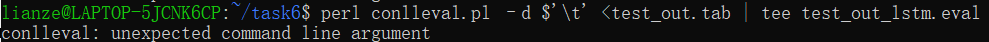
\includegraphics[scale=0.65]{./picture/error3.png} %1.png是图片文件的相对路径
  \caption{报错} %caption是图片的标题
  \label{asjhal} %此处的label相当于一个图片的专属标志,目的是方便上下文的引用
\end{figure}
经仔细检查,github上代码有误,原因在于-d的反斜杠是全角还是半角的问题,需要改成英文的斜杠“-”。\par
\subsection{评估结果}
\begin{figure}[H]
  \centering
  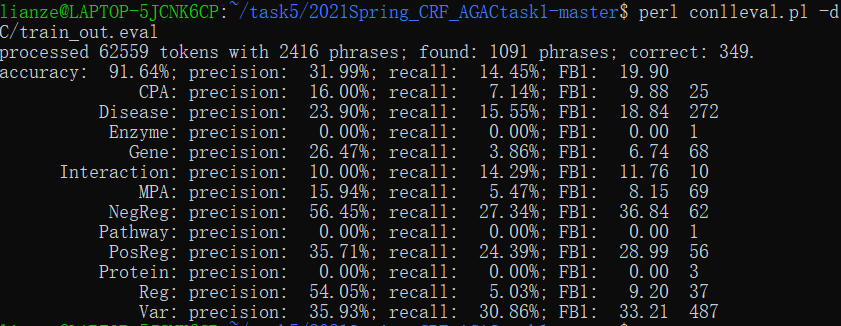
\includegraphics[scale=0.7]{./picture/result.png} %1.png是图片文件的相对路径
  \caption{最终评估结果} %caption是图片的标题
  \label{zzaa} %此处的label相当于一个图片的专属标志,目的是方便上下文的引用
\end{figure}
至此,我们本次LSTM+CRF训练模型、预测标签、评估结果一套流程全部完毕。可以看到预测的效果也比较一般,想要进一步提高效果,可以修改参数。例如循环次数。

\section{参考链接}
\begin{enumerate}
\item \href{http://www.qishunwang.net/news_show_69347.aspx}{\underline{Pytorch出现的小问题}}
\item \href{https://blog.csdn.net/weixin_44371912/article/details/109682671}{\underline{Rulcy的CSDN博客}}
\end{enumerate}


\end{document}


















%%%%%%%%%%%%%%%%%%%%%%%%%%%%Library%%%%%%%%%%%%%%%%%%%%%%%%%%%%%%%%%%%%%%%

% 1. 脚注用法
	LaTeX\footnote{Latex is Latex} is a good software

%2. 强调
	\emph{center of percussion} %[Brody 1986], %\lipsum[5]

%3. 随便生成一段话
	\lipsum[4]

%4. 列条目
	\begin{itemize}
	\item the angular velocity of the bat,
	\item the velocity of the ball, and
	\item the position of impact along the bat.
	\end{itemize}

%5. 表格用法
	\begin{table}[h]
	\centering  
	\begin{tabular}{c|cc}
		\hline
		年份 & \multicolumn{2}{c}{指标}\\
		\hline
		2017 & 0.9997 & 0.0555 \\
		2018 & 0.9994 & 0      \\
		2019 & 0.9993 & 0      \\
		\hline
	\end{tabular}
	\caption{NAME}\label{SIGN}
	\end{table}

	\begin{center}
		\begin{tabular}{c|cclcrcc}
			\hline
			Year & theta & $S_1^-$ & $S_2^-$ & $S_3^-$ & $S_4^+$ & $S_5^+$ & $S_6^+$ \\%表格标题
			\hline
			2016 & 1      & 0      & 0 & 0.0001 & 0      & 0      & 0 \\
			2017 & 0.9997 & 0.0555 & 0 & 0.2889 & 0.1844 & 0.463  & 0 \\
			2018 & 0.9994 & 0      & 0 & 0.0012 & 0.3269 & 0.7154 & 0 \\
			2019 & 0.9993 & 0      & 0 & 0      & 0.4325 & 1.0473 & 0 \\
			2020 & 0.9991 & 0      & 0 & 0      & 0.5046 & 1.2022 & 0 \\
			2021 & 0.999  & 0      & 0 & 0      & 0.5466 & 1.2827 & 0 \\
			2022 & 0.9989 & 0.0017 & 0 & 0.3159 & 0.562  & 1.2995 & 0 \\
			2023 & 0.9989 & 0      & 0 & 0.0109 & 0.5533 & 1.2616 & 0 \\
			2024 & 0.9989 & 0      & 0 & 0      & 0.5232 & 1.1769 & 0 \\
			2025 & 0.9989 & 0      & 0 & 0.1009 & 0.4738 & 1.0521 & 0 \\
			2026 & 0.9991 & 0      & 0 & 0      & 0.4071 & 0.8929 & 0 \\
			2027 & 0.9992 & 0.0004 & 0 & 0.1195 & 0.3248 & 0.7042 & 0 \\
			2028 & 0.9994 & 0.0164 & 0 & 0.046  & 0.2287 & 0.4902 & 0 \\
			2029 & 0.9997 & 0      & 0 & 0.0609 & 0.12   & 0.2545 & 0 \\
			2030 & 1      & 0      & 0 & 0      & 0      & 0      & 0 \\
			\hline
		\end{tabular}
	\end{center}

%6. 数学公式
	\begin{equation}
		a^2 = a * a\label{aa}
	\end{equation}
	
	\[
	\begin{pmatrix}{*{20}c}
	{a_{11} } & {a_{12} } & {a_{13} }  \\
	{a_{21} } & {a_{22} } & {a_{23} }  \\
	{a_{31} } & {a_{32} } & {a_{33} }  \\
	\end{pmatrix}
	= \frac{{Opposite}}{{Hypotenuse}}\cos ^{ - 1} \theta \arcsin \theta
	\]
	
	\[
	p_{j}=\begin{cases} 0,&\text{if $j$ is odd}\\
	r!\,(-1)^{j/2},&\text{if $j$ is even}
	\end{cases}
	\]
	
	
	\[
	\arcsin \theta  =
	\mathop{{\int\!\!\!\!\!\int\!\!\!\!\!\int}\mkern-31.2mu
		\bigodot}\limits_\varphi
	{\mathop {\lim }\limits_{x \to \infty } \frac{{n!}}{{r!\left( {n - r}
				\right)!}}} \eqno (1)
	\]

%7. 双图并行
	\begin{figure}[h]
		% 一个2*2图片的排列
		\begin{minipage}[h]{0.5\linewidth}
			\centering
			\includegraphics[width=0.8\textwidth]{./figures/0.jpg}
			\caption{Figure example 2}
		\end{minipage}
		\begin{minipage}[h]{0.5\linewidth}
			\centering
			\includegraphics[width=0.8\textwidth]{./figures/0.jpg}
			\caption{Figure example 3}
		\end{minipage}
	\end{figure}

%8. 单张图片部分
	\begin{figure}[h]
		%\small
		\centering
		\includegraphics[width=12cm]{./figures/mcmthesis-aaa.eps}
		\caption{Figure example 1} \label{fig:aa}
	\end{figure}

%%%%%%%%%%%%%%%%%%%%%%%%%%%%%%%%%%%%%%%%%%%%%%%%%%%%%%%%%%%%%%%%%%%%%%%%%%%%%
\begin{minipage}{0.5\linewidth}
	\begin{tabular}{|c|c|c|}
		\hline
		\multicolumn{2}{|c|}{\multirow{2}{*}{合并}}&测试\\
		\cline{3-3}
		\multicolumn{2}{|c|}{}& 0.9997  \\
		\hline
		2019 & 0.9993 & 0 \\
		\hline
	\end{tabular}
\end{minipage}

\begin{minipage}{0.5\linewidth}
	\begin{tabular}{c|ccc}
		\hline
		年份 & \multicolumn{3}{c}{指标}\\
		\hline
		\multirow{3}{*}{合并}&2017 & 0.9997 & 0.0555 \\
		&2018 & 0.9994 & 0      \\
		&2019 & 0.9993 & 0      \\
		\hline
	\end{tabular}
\end{minipage}



	\begin{table}[h]
	\centering	
	\begin{Large}
		\begin{tabular}{p{4cm} p{8cm} < {\centering}}
			\hline
			院\qquad 系: & 信息工程学院 \\
			\hline
			团队名称: & PlantBook Team \\
			\hline
			分\qquad 组: & 第0组1号 \\
			\hline
			日\qquad 期: & 2017年10月28日 \\
			\hline
			指导教师: & 吱吱吱\\
			\hline
		\end{tabular}
	\end{Large}
\end{table}


\ctexset{
	section={
		format+=\heiti \raggedright,
		name={,、},
		number=\chinese{section},
		beforeskip=1.0ex plus 0.2ex minus .2ex,
		afterskip=1.0ex plus 0.2ex minus .2ex,
		aftername=\hspace{0pt}
	},
}

	\begin{table}[h]
	\centering
	\begin{Large}
		\begin{tabular}{p{3cm} p{7cm}<{\centering}}
			院  \qquad  系: & 信息工程学院           \\ \cline{2-2}
		\end{tabular}
	\end{Large}		
\end{table}
\thispagestyle{empty}
\newpage
\thispagestyle{empty}
\tableofcontents
\thispagestyle{empty}
\newpage
\setcounter{page}{1}

% 9. 代码

\usepackage{listings}
\usepackage{xcolor}
\lstset{
	numbers=left, 
	numberstyle= \tiny, 
	keywordstyle= \color{ blue!70},
	commentstyle= \color{red!50!green!50!blue!50}, 
	frame=shadowbox, % 阴影效果
	rulesepcolor= \color{ red!20!green!20!blue!20} ,
	escapeinside=``, % 英文分号中可写入中文
	xleftmargin=2em,xrightmargin=2em, aboveskip=1em,
	basicstyle=\footnotesize,
	framexleftmargin=2em
}
